\documentclass[12pt,a4paper,danish,oneside]{book}
\setlength{\headheight}{15pt}
\usepackage{amsmath, amsthm, amssymb}
\usepackage[framemethod=default]{mdframed}
\usepackage{showexpl}
\usepackage[draft, danish]{fixme}

\mdfdefinestyle{exampledefault}{%
	rightline=true,innerleftmargin=10,innerrightmargin=10,
	frametitlerule=true,frametitlerulecolor=green,
	frametitlebackgroundcolor=yellow,
	frametitlerulewidth=2pt}

\usepackage{lipsum}
\usepackage[framed,numbered,autolinebreaks,useliterate]{mcode}
\usepackage{minted}
\usepackage{url,textcomp}
\usepackage{graphicx}
\usepackage[danish]{babel}
\usepackage[utf8x]{inputenc}
\usepackage{siunitx}
\usepackage{caption}
\usepackage{float}
\usepackage{gensymb}

\newmdtheoremenv{exmp}{Example}[section]
\newtheorem{prob}{Problem}[section]
\setcounter{section}{1}


\usepackage{titlesec}
\titleformat{\chapter}[display]
{\normalfont\bfseries\filcenter}
{}
{1ex}
{\titlerule[2pt]
\vspace{2ex}%
\LARGE}
[\vspace{1ex}%
{\titlerule[2pt]}]


\usepackage{cancel}
\usepackage[margin=4cm]{geometry}
\usepackage[hidelinks]{hyperref}
\usepackage{cleveref}
\usepackage{enumitem}
\usepackage{fancyhdr}
\pagestyle{fancy}
\fancyhead{}
\fancyfoot{}
\lhead{ETLYAK}
\rhead{\textsc{Jonas Lind}}
\cfoot{\thepage}
    
\newcommand{\HRule}{\rule{\linewidth}{0.5mm}}



\title{ETLYAK - Sound and Acoustics}
\begin{document}
\begin{titlepage}
	\clearpage\thispagestyle{empty}

	\begin{center}
		\HRule \\[0.4cm]
		{\huge \bfseries ETLYAK} \\[.3cm] {\huge Lyd og Akustik}\\[0cm]		
		\HRule \\[3.4cm]
		
\includegraphics[width=0.5\linewidth]{graphics/au}
	\end{center}
	\renewcommand{\contentsname}{Indholdsfortegnelse}
	\tableofcontents

\end{titlepage}
 
%-----------------------------------------------------------------
%   TITLE SECTION
%-----------------------------------------------------------------
\listoffixmes

\chapter{Karakterisering af lyd}
\section{Lektion 15-02-2018}
\subsection{GraphicTFT display driver}

Driver for "ITDB02 320 x 240 TFT display module, Version 2" mounted at "ITDB02 Arduino Mega2560 Shield".\\

\noindent Display controller = ILI 9341.\\

\begin{tabular}{ll}
	\textbf{Connections}\\
	\hline
	\rule{0pt}{5mm}  
	DB15-DB8:   & PORT A\\ 
	\rule{0pt}{5mm}
	DB7-DB0:    & PORT C\\ 
	\rule{0pt}{5mm}
	RESETx:     & PORT G, bit 0\\ 
	\rule{0pt}{5mm}
	CSx:        & PORT G, bit 1\\ 
	\rule{0pt}{5mm}
	WRx:        & PORT G, bit 2\\ 
	\rule{0pt}{5mm}
	RS (=D/Cx): & PORT D, bit 7\\ 
\end{tabular} 

\begin{minted}{c}
// Data port definitions:
#define DATA_PORT_HIGH PORTA
#define DATA_PORT_LOW  PORTC

// Control port definitions:
#define WR_PORT PORTG
#define WR_BIT 2
#define DC_PORT PORTD
#define DC_BIT  7  // SHIELD RS
#define CS_PORT PORTG
#define CS_BIT  1
#define RST_PORT PORTG
#define RST_BIT 0
\end{minted}
Start by implementing the basic, time-critical functions.

\begin{figure} [H]
	\centering
	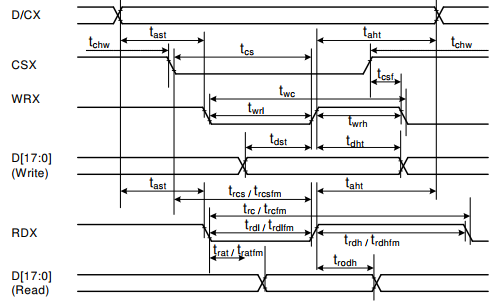
\includegraphics[width=0.8\linewidth]{graphics/LAB3a.png}
	\caption{Timing Characteristics (8080-Ⅰ system).}
	\label{fig:11}
\end{figure}

\noindent\mintinline{c}{PORTD &= ~(1 << n);} will set PIN n low.\\

\noindent\mintinline{c}{PORTD |= (1 << n);} will set PIN n high.

\begin{minted}{c}
void WriteCommand(unsigned int command)
{
DATA_PORT_LOW = command;
DC_PORT &= ~(1<<DC_BIT);       // DCX LOW = COMMAND MODE
CS_PORT &= ~(1<<CS_BIT);       // CSX LOW
WR_PORT &= ~(1<<WR_BIT);       // WRX LOW
_NOP();			// DELAY = twrl 15ns
WR_PORT |= (1<<WR_BIT);	// WRX HIGH
_NOP();			// DELAY = tcf 10ns
}
\end{minted}

\begin{minted}{c}
void WriteData(unsigned int data)
{
DATA_PORT_HIGH = (data >> 8);	// MSB
DATA_PORT_LOW  = data;	       // LSB
DC_PORT |= (1<<DC_BIT);	      // DCX HIGH = DATA MODE
CS_PORT &= ~(1<<CS_BIT);	     // CSX LOW
WR_PORT &= ~(1<<WR_BIT);	     // WRX LOW
_NOP();			      // DELAY = twrl 15ns
WR_PORT |= (1<<WR_PORT);	     // WRX HIGH
_NOP();			      // DELAY = twcf 10ns
}
\end{minted}

\chapter{Måling/Opsamling af lyd}
\section{Lektion 08-02-2018}

\begin{enumerate}
	\item Mikrofon
	\item Højtaler (afstandsregel)
	\item Måling af lydtryk
\end{enumerate}

\begin{mdframed}[style=exampledefault]
	\begin{itemize}
		\item \textbf{Pensum:} 
		\begin{enumerate}
			\item Audio Meetering, sec. 8-9, 26-29
			\item Elektroakustik, TAS,  p. 12-14
		\end{enumerate}
		\item \textbf{Opgaver:} 
		\begin{enumerate}
			\item Lyd og Akustik - Lektion 2 - opgaver og øvelser
		\end{enumerate}
	\end{itemize}
\end{mdframed}

\subsection{Mikrofon}
\begin{itemize}
	\item En transducer der omsætter et oscillerende lydtryk til et analogt elektrisk signal.
	\begin{itemize}
		\item Kaldes også for en tryktransducer.
		\item Måler lydtrykkets variation i et punkt uden reference til den retning lyden udbredes i.
		\item Flere mikrofontyper er retningsbestemte på grund af deres opbygning.
	\end{itemize}
\end{itemize}

\subsubsection{Kondensator mikrofon}
\begin{itemize}
	\item En tynd membran af udspændt metalfolie er anbragt tæt på
	en fastsiddende elektrode.
	\item Kondensatoren mellem membran og elektrode oplades gennem $R_p$. 
	\item Spændingen mellem membran og elektrode vil variere efter definitionsligningen $Q = C\cdot U$.
	\begin{itemize}
		\item $Q$ er den konstante ladning givet af polarisationsspændingen $U_P$ der ved målemikrofoner typisk er \SI{200}{\volt}.
	\end{itemize}
	\item Den lave grænsefrekvens sættes af $R_p$ og mikrofonens kapacitet $C$.
	\begin{itemize}
		\item $C \approx \SI{5}{\pico\farad}-\SI{20}{\pico\farad}$ gør at  $R_p$ skal være mindst \SI{1}{\giga\ohm} for måling af hørbar lyd.
	\end{itemize}
	\item Den høje grænsefrekvens sættes af membranens masse. 
\end{itemize}

\begin{figure} [H]
	\centering
	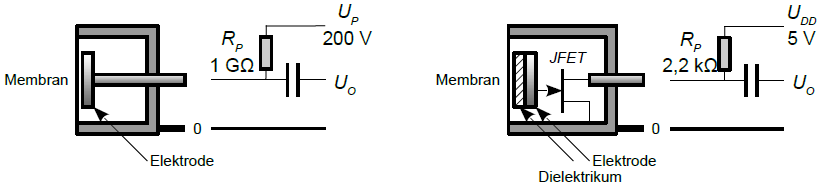
\includegraphics[width=\linewidth]{graphics/11.png}
	\caption{Kondensatormikrofons opbygning.}
	\label{fig:11}
\end{figure}

\begin{itemize}
	\item Alternativt indbygges en plastskive mellem membran og elektrode hvor en såkaldt "fastfrosset ladning" fungerer som $Q$.
	\item Den høje udgangsimpedans sænkes af en indbygget JFET og det eksterne kredsløb skal nu levere strøm til transistorens drain.
	\item Følsomheden er typisk $\approx 5 \si{\milli\volt}/\si{\pascal}$. 
\end{itemize}

\subsubsection{Dynamisk mikrofon}
\begin{itemize}
	\item \textbf{Klassiske form}: minder om en højttaler (membranen sættes i bevægelse af lydtrykket). Derved bevæges svingspolen i magnetfeltet
	og der induceres en spænding.
	\item \textbf{Båndmikrofonen}: membranen er i et kraftigt magnetfelt. Når lydtrykket får membranen til at svinge induceres der en spænding over de to ender af båndet. Spændingen er normalt så lav at der skal benyttes en transformator for at løfte det op på et brugbart niveau. 
	\begin{itemize}
		\item Lyden har adgang til begge sider af membranen.
		\begin{itemize}
			\item Mest følsom for lyd på aksen ($0\degree$ og $180\degree$.
			\item Der kan ikke registreres lyd fra siden ($90\degree$).
		\end{itemize}
	\end{itemize} 
\end{itemize}
\begin{figure} [H]
	\centering
	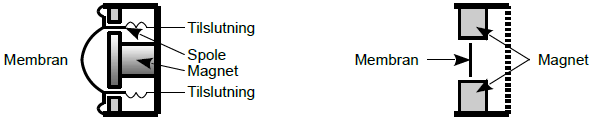
\includegraphics[width=.9\linewidth]{graphics/12.png}
	\caption{(V: svingspolen drives af en membran til at svinge i et magnetfelt.) (H: En tynd metalfolie svinger i et magnetfelt og signalet tages ud ved båndets ender (ud af papiret og ind i papiret)).}
	\label{fig:12}
\end{figure}

\subsection{Højtaler (afstandsregel)}
\fxnote{Mangler højtaler (aftandsregel) noter.}

\subsection{Måling af lydtryk}
\fxnote{Mangler måling af lydtryk noter.}

\subsection{Opgaver}

\begin{enumerate}
	\item Lav et MLS signal med orden 10.
	\item Find impulsresponsen ud fra de sammenhørende exitations- og målesignaler i filen meassigs.mat. Systemet er ”målt” både med MLS og hvid støj.
	\item En 8 ohms højttaler har DC modstand på 6 ohm og virkningsgrad på 1 \%.
	\begin{enumerate}
		\item Bestem den producerede akustiske effekt, når højttaleren tilføres 2,83 volt.
		\item Lyden antages at udbrede sig sfærisk fra højttaleren. Beregn intensiteten og lydtrykniveauet på 2,5 meters afstand.
		\item Lydtrykket måles nu med en mikrofon hvis følsomhed er 5 mV/Pa. Hvilken spænding leverer mikrofonen?
	\end{enumerate}
\end{enumerate}


\begin{lstlisting}
%% LYAK L2 08-02-2018

\end{lstlisting}



\chapter{Psykoakustik - Menneskets opfattelse af lyd}
\section{Lektion 15-03-2018}

\begin{enumerate}
	\item Ørets opbygning
	\item Frekvensopfattelse
	\item Lydniveau
	\item Lokalisering af lydkilder (retningsbestemmelse)
\end{enumerate}

\begin{mdframed}[style=exampledefault]
	\begin{itemize}
		\item \textbf{Pensum:} 
		\begin{enumerate}
			\item Master Handbook Of Acoustics, ch. 4
			\item Audio Meetering, sec. 7, 10
			\item Elektroakustik, TAS,  p. 7-11
		\end{enumerate}
		\item \textbf{Opgaver:} 
		\begin{enumerate}
			\item Lyd og Akustik - Lektion 3 - opgaver og øvelser
		\end{enumerate}
	\end{itemize}
\end{mdframed}
\fxnote{Mangler psykoakustik noter.}
\subsection{Ørets opbygning}
\subsection{Frekvensopfattelse}
\subsection{Lydniveau}
\subsection{Lokalisering af lydkilder}
\subsubsection{Retningsbestemmelse}

\chapter{Lydens opførsel i lukkede rum}
\section{Lektion 15-02-2018}

\begin{enumerate}
	\item Stående bølger
	\item Geometrisk rumakustik
	\item Refleksion
	\item Diffraktion
	\item Statistisk rumakustik
	\item Absorptionskoeffficienter
\end{enumerate}

\noindent\fbox{\parbox{\textwidth}{
	\begin{itemize}
	\item \textbf{Pensum:} 
	\begin{enumerate}
		\item Master Handbook of Acoustics, ch. 6, 7, 11, 13
		\item Elektroakustik, TAS,  p. 89-96
	\end{enumerate}
	\item \textbf{Opgaver:} 
	\begin{enumerate}
		\item Lyd og Akustik - Lektion 4 - opgaver og øvelser
	\end{enumerate}
\end{itemize}
}} \vspace{3mm}

\subsection{Stående bølger}
Et retvinklet rum vil have et system af egenfrekvenser. Her vil plane bølger spejles så de understøtter bestemte frekvenser. Dette sker gennem konstruktiv interferens. \\

\noindent Den laveste frekvens hvor der kan dannes resonans i en akseretning har en bølgelængde på halvdelen af længdedimensionen ($L_x$, $L_y$ og $L_z$). Trykbølgen reflekteres ved væggen og refleksionen kan derfor understøtte den efterfølgende bølgefront.
\begin{itemize}
	\item Ved \SI{5}{\meter} afstand mellem to vægge er den lavest mulige resonans $f_0 = \SI{34}{\hertz}$. Hertil kommer også resonans ved de harmoniske frekvenser på \SI{68}{\hertz}, \SI{102}{\hertz}, ... Tilsvarende gælder for de andre akseretninger.
\end{itemize}
Der er mulighed for stående bølger som involverer fire eller seks vægge.
Dette beskrives ved at to eller tre værdier af index ($n_x$, $n_y$ og $n_z$) er forskellige fra nul. 
De tre indeksværdier kombineres til et enkelt ved at udnytte at N er den højest mulige værdi. Herved kan resonanserne plottes som
funktion af et fælles indeks \textit{n}.\\

\noindent Modellen gælder indtil frekvenser hvor usikkerheden på længderetningen
bliver sammenlignelig med bølgelængden. 
Det kan vises at den øvre grænse er i cirka \SI{550}{\hertz} for
et normalt beboelsesrum hvorved det enkelte indeks er begrænset til området $n = 0$ ... $7$.

\begin{figure} [H]
	\centering
	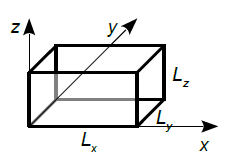
\includegraphics[width=.4\linewidth]{graphics/13.png}
	\caption{Plane lydbølger kan eksistere i et rektangulært rum.}
	\label{fig:13}
\end{figure}
\noindent\textbf{Resonanser}
\begin{equation}
f_n = \sqrt{\left(\dfrac{n_x c}{2 L_x}\right)^2 + \left(\dfrac{n_y c}{2 L_y}\right)^2 + \left(\dfrac{n_z c}{2 L_z}\right)^2}
\end{equation}

\noindent\textbf{Øvre grænse}
\begin{equation}
f_{max}\approx \dfrac{c}{2\pi \Delta L}
\end{equation}

\begin{equation}
N \approx 1 +\dfrac{V}{S \Delta L}
\end{equation}

\begin{description}
	\item[$V$] rummets volume $m^3$
	\item[$\Delta L$] længdedimensionen
	\item[$S$] lydabsorberende areal
\end{description}
\newpage
\begin{itemize}
	\item Ved lave frekvenser er det let at adskille de enkelte resonanser.
	\item Ved højere frekvenser rykker resonanserne sammen og flere resonanser vil blive aktiveret i større eller mindre grad af en stationær tone. 
	\item Når centerfrekvensen af et antal	resonanser falder indenfor båndbredden af det enkelte filter er det umuligt at skelne mellem
	egenfrekvenserne.
	\item Grænsefrekvensen mellem det område hvor de enkelte resonanser kan erkendes og det område	hvor de er smeltet sammen kaldes for Schröder frekvensen. 
	\item Findes fra rummets volumen $V$ og efterklangstid $T_{60}$. Teorien antager at der vil ligge mindst	tre resonanser indenfor det midterste filters $–3 \si{\decibel}$ båndbredde.
\end{itemize}

\begin{equation}
f_s = 2000 \sqrt{\dfrac{T_{60}}{V}}
\end{equation}

\begin{itemize}
	\item Rummets resonanser er ansvarlig for efterklangen i rummet.
	\item En højttaler udsender	et støjsignal der indeholder alle frekvenser så samtlige resonanser i rummet aktiveres. 
	\item Når lydniveauet er blevet konstant standses lyden fra højttaleren og lydniveauet aftager i takt med at lydenergien absorberes i tæpper, træpaneler og vinduer samt luften selv.
	\item Efterklangstiden $T_{60}$ er defineret som tiden indtil signalet er reduceret til \SI{-60}{\decibel} af det oprindelige niveau.
	\item Resonanserne kan beskrives ved dæmpede svingninger der fra filterteorien repræsenteres af et anden-ordens filter for hver resonans.
\end{itemize}

\begin{equation}
H(s)=\sum_{n=0}^{N}\dfrac{C_n}{s^2+2d_n\omega_n s+\omega_n^2}
\end{equation}

\begin{equation}
h(t)=\sum_{n=0}^{N} C_n \sin(\omega t) \exp(-d_n\omega_n t)
\end{equation}

\subsection{Geometrisk rumakustik}
En lydbølge fra lydgiveren udbredes med en konstant hastighed i alle retninger. 
En lytter i nogen afstand fra lydgiveren vil modtage lydbølgen efter en forsinkelse $t_D$ på cirka $3 \si{\milli\second}$ per meter.\\

\noindent Lydbølgen vil fortsætte sin udbredelse indtil den rammer en flade i rummet hvor den reflekteres og den reflekterede bølgefront kan derfor nå frem til lytteren efter yderligere forsinkelse. 
Øret vil modtage et system af lydbølger der både beskriver det materiale der lyttes på og det rum lydkilden og personen befinder sig i.
\subsubsection{Refleksion}
\begin{itemize}
	\item Et rums impulsrespons kan beregnes ved at følge de veje som refleksionerne vil løbe. Resultatet bliver kun en tilnærmelse uanset hvor omhyggeligt der beregnes.
	\item En refleksion forløber ikke med stor præcision. Der opstår en udtværing af det reflekterede signals retning som nu spredes i enhver retning og ikke alene er givet af signalets ind- og udfaldsvinkler.
	\item Den direkte spejling står for cirka 80 \% af energien i den
	indfaldne bølgefront og den diffuse udstråling i enhver retning står for den resterende energi.
	\item Som model af den diffuse stråling anvendes statistiske metoder for at ændre lidt på refleksionens retning i forhold til en direkte spejling.
\end{itemize}

\begin{figure} [H]
	\centering
	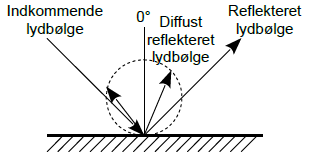
\includegraphics[width=.55\linewidth]{graphics/14.png}
	\caption{En lydbølges refleksioner sker både som en direkte spejling af lydbølgen og som en diffus lydbølge.}
	\label{fig:14}
\end{figure}

\subsubsection{Diffraktion}
Hvordan lydbølger bøjes af små forhindringer og hvordan lydbølger udbredes efter små åbninger. 

\begin{itemize}
	\item En forhindring meget smallere end lydbølgen gør at lydbølgen kan passere uden at blive synderligt forstyrret.
	\item En forhindring større end lydbølgen vil resultere i at der bliver kastet en skygge (casts a shadow) der vil  blive bestrålet fra kilder, der går forbi forhindringen.
\end{itemize}

\begin{figure} [H]
	\centering
	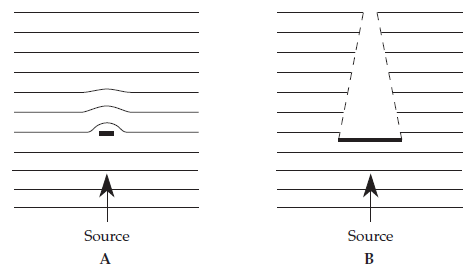
\includegraphics[width=.5\linewidth]{graphics/15.png}
	\caption{Diffraktion er wavelength-dependent.}
	\label{fig:15}
\end{figure}

\begin{itemize}
	\item Diffraktionen afhænger af	den relative størrelse af åbningen. 
	\item En stor åbning med hensyn til bølgelængde tillader lydbølger at gå igennem med en lille forstyrrelse. 
	\begin{itemize}
		\item Disse bølgefronter virker som nye kilder, der udstråler lydenergi i skyggezonen.
	\end{itemize}
	\item Hvis åbningen er lille i forhold til bølgelængden, vil de små bølgefronter, der trænger ind i åbningen virke som punktkilder.
	\begin{itemize}
		\item Disse små bølgefronter vil udstråle et halvkugleformet lydfelt ind i skyggezonen.
	\end{itemize} 
\end{itemize}

\begin{figure} [H]
	\centering
	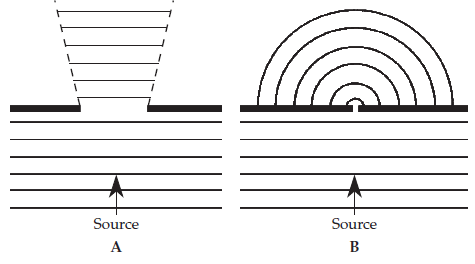
\includegraphics[width=.5\linewidth]{graphics/16.png}
	\caption{Lydbølger der rammer en barriere med en åbning.}
	\label{fig:16}
\end{figure}


\subsection{Statistisk rumakustik}
\begin{itemize}
	\item Antager at lydenergien er konstant overalt i rummet.
	\item \textbf{Sabines formel} for efterklangstiden $T_{60}$ som funktion af rummets volumen V og det lydabsorberende areal S.
\end{itemize}

\begin{equation}
T_{60} = \ln(10^6)\dfrac{4V}{S c} = 55.3\dfrac{V}{S c} = 0.16\dfrac{V}{S}
\end{equation}

\begin{itemize}
	\item For lyddæmpede rum giver Sabines formel en efterklangstid selv om der ikke er refleksioner. En modificeret udgave af Sabines formel blev udledt af Eyring.
	\item \textbf{Eyrings formel} er modificeret ud fra geometriske betragtninger.
\end{itemize}

\begin{equation}
T_{60} = 0.16\dfrac{V}{4 m V-S\ln(1-\alpha)}
\end{equation}

\begin{description}
	\item[$\alpha$] $=\frac{1}{S}\sum_{n}^{}S_n \alpha_n$
	\item[$m$] $\approx0.0011 m^{–1}$ ved \SI{1}{\kilo\hertz}, \SI{20}{\degreeCelsius} og 60 \% relativ luftfugtighed
\end{description}
\textit{m} kan ignoreres for mindre rum og rum med ringe dæmpning bliver formlen lig med Sabines.

\subsection{Absorptionskoeffficienter}
\begin{itemize}
	\item Typisk opsætning af lydabsorberende skumplast og Rockwool er direkte på en hård betonvæg.
	\item Tykkelsen er afgørende for hvor lave frekvenser der kan dæmpes da partikelhastigheden er nul ved væggen så det er kun	ved høje frekvenser at der er bevægelse i luften inde i materialet.
	\item For at opnå større absorption ved lave frekvenser kan benyttes absorbere baseret på en membran.
	\begin{itemize}
		\item De består af en plade eller film af træ, plast eller metal som lydtrykket får til at vibrere.
		\item Derved skal luften bag ved membranen også svinge så luften presses igennem det absorberende materiale.
	\end{itemize}
\end{itemize}


\chapter{Virtuel akustik - Spejlkildemodel}
\section{Lektion 22-02-2018}

\begin{enumerate}
	\item Virtuel Akustik
	\item Ray Tracing Method
	\item Image Source Method
	\item Reflektogram
\end{enumerate}

\begin{mdframed}[style=exampledefault]
	\begin{itemize}
		\item \textbf{Pensum:} 
		\begin{enumerate}
			\item The Use of Computer Modeling in Room Acoustics, \\J. H. Rindel
			\item Image Method For Efficiently Simulating Small-Room\\ Acoustics, Jont B. Allen and David A. Berkley
		\end{enumerate}
		\item \textbf{Opgaver:} 
		\begin{enumerate}
			\item Lyd og Akustik - Lektion 5 - opgaver og øvelser
		\end{enumerate}
	\end{itemize}
\end{mdframed}

\subsection{Virtuel Akustik}
\begin{itemize}
	\item Audio for virtual reality has many equivalent	terms, such as auralization, virtual acoustics, binaural room simulation and auditory display.
	\item Common approach to auralization is a two-stage process:
	\begin{itemize}
		\item Computation of an impulse response (IR) representing an acoustic space.
		\item Convolution of this impulse response with a dry (anechoically
		recorded or synthetically generated) source signal.
	\end{itemize} 
\end{itemize}

\subsection{Ray Tracing Method}
\begin{itemize}
	\item Den samlede energi der udsendes af en source er fordelt som stråler i et bestemt antal af retninger.
	\item Energien af hver enkel stråle er lig med den samlede energi delt med antallet stråler. 
	\item Afhængig af overfladens absorption vil hver stråle spejles med indfaldsvinklen er lig med vinklen på refleksionen eller diffus reflekteret, hvor retningen af den reflekterede stråle er randomiseret.
	\item For at opnå et beregningsresultat relateret til en bestemt
	receiver position \textit{R1} er det nødvendigt at definere et område eller en volumen omkring receiveren for at fange strålerne.
	\item Der er en risiko for beregne falske refleksioner og at nogle mulige refleksioner ikke findes.
\end{itemize}

\begin{figure} [H]
	\centering
	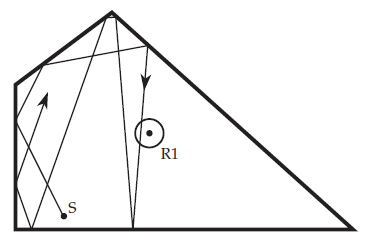
\includegraphics[width=.6\linewidth]{graphics/17.png}
	\caption{Ray Tracing - source S, receiver area R1.}
	\label{fig:17}
\end{figure}

\subsection{Image Source Method}
\begin{itemize}
	\item Et virtuelt image af den faktiske kilde (real source) bestemmes ved at reflektere kilden vinkelret på tværs af en rumgrænse (boundary).
	\item Den virtuelle kilde (image source) er placeret i en afstand \textit{d} der svarer til den dobbelte afstand mellem source og rumgrænsen (vinkelret).
	\item Afstanden mellem den virtuelle kilde S1 og receiveren R1 svarer til refleksions distancen (reflection path) mellem S og R1.
	\item Refleksionerne af alle reelle og virtuelle kilder, der krydser en rumgrænse, skaber et mirror image.
	\item Ved et rekangulært rum vil alle virtuelle kilder være synlige i alle positioner i rummet og beregningen er hurtig.
	\item Gælder ikke ved irregulære rum. Validering af hvert image er påkrævet og antallet af beregninger bliver hurtigt mange.
	\item 2. ordens refleksion når en stråle rammer 2 rumgrænser inden den når receiveren.
\end{itemize}

\begin{figure} [H]
	\centering
	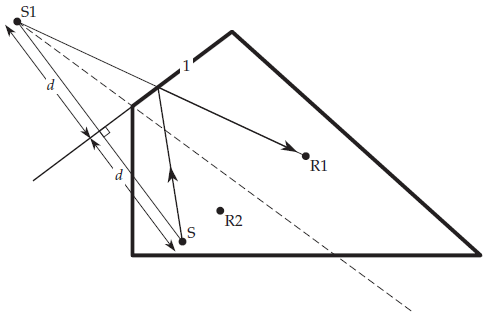
\includegraphics[width=.75\linewidth]{graphics/18.png}
	\caption{ISM - real source S, virtual source S1, receiver R1.}
	\label{fig:18}
\end{figure}

\noindent Estimat af antallet \textit{N} refleksioner som receiveren vil modtage indenfor tiden \textit{t}.

\begin{equation}
N_{refl}=\dfrac{4\pi c^3}{3V}t^3
\end{equation}

\noindent Ved \textit{n} antal rumgrænser = \textit{n} antal mulige 1. ordens image sources som kan medføre \textit{n-1} 2. ordens image sources. \\

\noindent Estimat af mulige image sources ved \textit{i} ordens image source. 

\begin{equation}
N_{sou}=1+\dfrac{n}{(n-2)}((n-1)^i -1)\approx (n-1)^i
\end{equation}

\newpage
\subsection{Reflektogram}
\begin{itemize}
	\item Viser ankomsten af tidlige refleksioner til en receiver.
	\item Arrival time (\textit{x-aksen}) og energi af refleksionen (\textit{y-aksen}).
\end{itemize}

\begin{figure} [H]
	\centering
	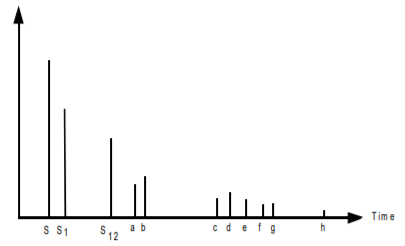
\includegraphics[width=.75\linewidth]{graphics/19.png}
	\caption{Reflectogram for receiver R med 2 image sources.}
	\label{fig:19}
\end{figure}

\subsection{Øvelser}
\begin{enumerate}
	\item \textbf{Øvelse 5.1:} Modeller et virtuelt rum vha. spejlkildemetoden. Bestem selv rummets dimensioner, absorbtions-koefficienter for overfladematerialerne (keep it simple) og position af lydkilde og modtager. Generer et reflektogram h1(n) fra en tænkt lydkilde (fast position) til en modtager. Modelleringsorden N bør ikke overstige 10 – det skulle dække alle tidlige reflektioner.
	\item \textbf{Øvelse 5.2:} Lav et estimat af efterklangstiden for det virtuelle rum i øvelse 5.1 via Sabine’s formel og konstruer dernæst en efterklangshale (eksponentielt vægtet hvid støj), som hægtes efter h1(n). Så får vi et væsentligt længere reflektogram h2(n). Hvad mangler for at h2(n) ligner en ”rigtig” målt impulsrespons?
\end{enumerate}


\begin{lstlisting}
%% LYAK L5 22-02-2018

\end{lstlisting}


\chapter{Virtuel akustik - Auralisation}
\section{Lektion 06-03-2018}

\begin{enumerate}
	\item Impedans tilpasning
	\item L kredsløb
	\item Pi kredsløb
	\item T kredsløb
\end{enumerate}

\begin{mdframed}[style=exampledefault]
	\begin{itemize}
		\item \textbf{Pensum:} CB, Ch 4 p. 63-72
		\item \textbf{Opgaver:} Lektion 4-1, Lektion 4-2, Lektion 4-3
	\end{itemize}
\end{mdframed}

\noindent\textit{Impedance matching is often necessary in the design of RF circuitry to provide the maximum possible transfer of power	between a source and its load.}

\subsection{L kredsløb}

\begin{itemize}
	\item 4 mulige kombinationer af placeringen af L og C komponenterne.
	\begin{itemize}
		\item 2 kombinationer der resulterer i en lavpas konfiguration.
		\item 2 kombinationer der resulterer i en højpas konfiguration.
	\end{itemize}
\end{itemize}

\subsubsection{Analysis}
\begin{itemize}
	\item Determine what the load impedance actually looks
	like when the capacitor is placed across the load resistor.
\end{itemize}

\begin{equation}
Z = \dfrac{X_C R_L}{X_C+R_L}
\end{equation}

\begin{itemize}
	\item The parallel combination of the capacitor and resistor looks like an impedance in series.
	\item To complete the impedance match to source resistance is to add an equal and opposite reactance in series.
	\item The addition of the inductor causes cancellation of the capacitor leaving only an apparent load resistor.
	\begin{itemize}
		\item The shunt component of the impedance-matching network is to transform a larger impedance downto a smaller value with a real part equal to the real part of the other terminating impedance.
		\item The series impedance-matching element then resonates with or cancels any reactive component present, thus leaving the source driving an apparently equal load for optimum power transfer.
	\end{itemize}
\end{itemize}


\begin{figure} [H]
	\centering
	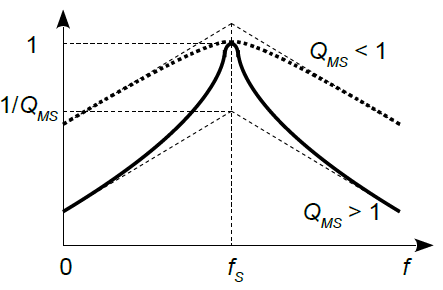
\includegraphics[width=0.8\linewidth]{graphics/26.png}
	\caption{L network.}
	\label{fig:26}
\end{figure}

\newpage\subsubsection{Design}

\begin{itemize}
	\item $X_p$ and $X_s$ may be either capacitive or inductive reactance but each must be of the opposite type. Once $X_p$ is chosen as a capacitor, for example, $X_s$ must be an inductor, and vice versa.
\end{itemize}

\begin{equation}
Q_s = Q_p = \sqrt{\dfrac{R_p}{R_s}-1}
\end{equation}

\begin{equation}
Q_s = \dfrac{X_s}{R_s}
\end{equation}

\begin{equation}
Q_p = \dfrac{R_p}{X_p}
\end{equation}

\begin{description}
	\item[$Q_s$] Q of the series leg
	\item[$Q_p$] Q of the shunt leg
	\item[$R_p$] shunt resistance
	\item[$X_p$] shunt reactance
	\item[$R_s$] series resistance
	\item[$X_s$] series reactance
\end{description}

\subsubsection{Complex loads}
Two basic approaches in handling complex impedances.
\begin{itemize}
	\item Absorption
	\begin{itemize}
		\item Absorb any stray reactances into the impedance-matching network itself.
		\item Done through placement of each matching element such that element capacitors are placed in parallel with stray capacitances.
		\item Element inductors are placed in series with any stray inductances. 
		\item Stray component values are subtracted from the calculated element
		values, leaving new element values (C', L'), smaller than the calculated element values.
	\end{itemize}
	\item Resonance
	\begin{itemize}
		\item Resonate any stray reactance with an	equal and opposite reactance at the frequency of interest.
	\end{itemize}
\end{itemize}

\subsection{Pi kredsløb}
\textit{Two "back-to-back" L networks that are both configured to match the load and
	the source to an invisible or "virtual" resistance located at the junction between the two networks.}

\begin{figure} [H]
	\centering
	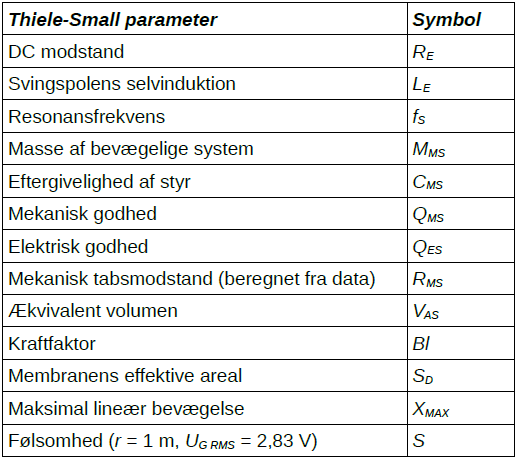
\includegraphics[width=0.6\linewidth]{graphics/27.png}
	\caption{Three element Pi network.}
	\label{fig:27}
\end{figure}

\begin{itemize}
	\item The negative signs for $-X_{s1}$ and $-X_{s2}$ is symbolic.
	\item Used to indicate that the $X_s$ values are the opposite type of reactance from $X_{p1}$ and $X_{p2}$.
\end{itemize}

\begin{figure} [H]
	\centering
	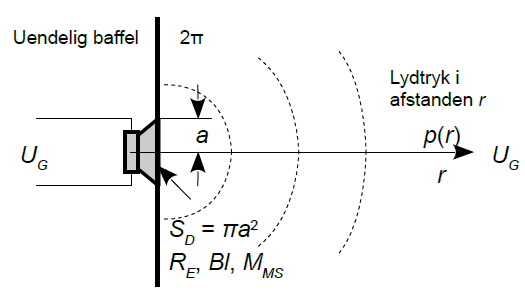
\includegraphics[width=0.8\linewidth]{graphics/29.png}
	\caption{Pi network shown as two back-to-back L networks.}
	\label{fig:29}
\end{figure}

\subsubsection{Design}
\begin{itemize}
	\item The virtual resistance (\textit{R}) must be smaller than either $R_s$ or $R_L$.
	\item Most of the time, \textit{R} is defined by the desired loaded \textit{Q} of the
	circuit that you specify.
\end{itemize}

\begin{equation}
Q = \sqrt{\dfrac{R}{R_{small}}-1}
\end{equation}


\subsection{T kredsløb}
\textit{The T network is often used to match two low-valued impedances when a high-Q arrangement is needed.}

\begin{figure} [H]
	\centering
	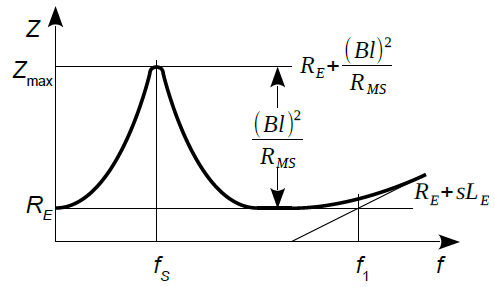
\includegraphics[width=0.6\linewidth]{graphics/28.png}
	\caption{Three element T network.}
	\label{fig:28}
\end{figure}

\noindent\textit{The Pi and T networks are great for narrow-band matching networks.\\
What if an impedance match is required over a fairly broad range of frequencies?}

\begin{itemize}
	\item Two series-connected L sections rather than the back-to-back configuration
	of the Pi and T networks.
	\begin{itemize}
		\item Value of the virtual resistor (R) must be larger than the smallest termination impedance and smaller than the largest termination
		impedance.
	\end{itemize}
	\item Maximum bandwidth (minimum Q) available:
\end{itemize}

\begin{equation}
R = \sqrt{R_S R_L}
\end{equation}

\begin{equation}
Q = \sqrt{\dfrac{R}{R_{smaller}-1}}= \sqrt{\dfrac{R_{larger}}{R}-1}
\end{equation}

\begin{description}
	\item[$R$] virtual resistance
	\item[$R_{smaller}$] smallest terminating resistance
	\item[$R_{larger}$] largest terminating resistance
\end{description}

\noindent\textit{If even wider bandwidths are needed, more L networks may be	cascaded with virtual resistances between each network.}
\begin{equation}
\dfrac{R_1}{R_{smaller}} = \dfrac{R_2}{R_1}= \dfrac{R_3}{R_2} ... = \dfrac{R_{larger}}{R_n}
\end{equation}

\begin{figure} [H]
	\centering
	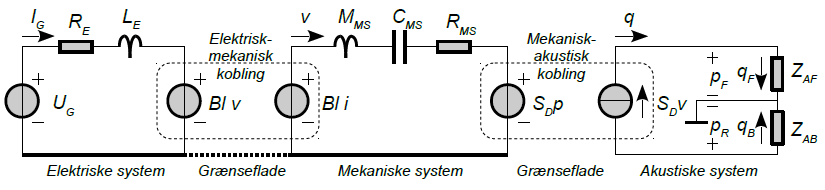
\includegraphics[width=0.8\linewidth]{graphics/30.png}
	\caption{Two series-connected L networks for lower Q applications.}
	\label{fig:30}
\end{figure}

\chapter{Gengivelse af lyd}
\section{Lektion 22-03-2018}

\begin{enumerate}
	\item Højttalerens model
	\item Elektrisk
	\item Mekanisk
	\item Akustisk
\end{enumerate}

\noindent\fbox{\parbox{\textwidth}{
	\begin{itemize}
	\item \textbf{Pensum:} 
	\begin{enumerate}
		\item Elektroakustik, TAS,  p. 29-41
	\end{enumerate}
	\item \textbf{Opgaver:} 
	\begin{enumerate}
		\item Lyd og Akustik - Lektion 7 - opgaver og øvelser
	\end{enumerate}
\end{itemize}
}} \vspace{3mm}

\subsection{Højttalerens model}
\begin{itemize}
	\item Er en transducer som omsætter elektrisk energi til akustisk energi.
	\item Benytter en let og stiv membran som sættes i bevægelse af en elektromagnetiske kraft for at overføre energi til luften.
\end{itemize}

\begin{figure} [H]
	\centering
	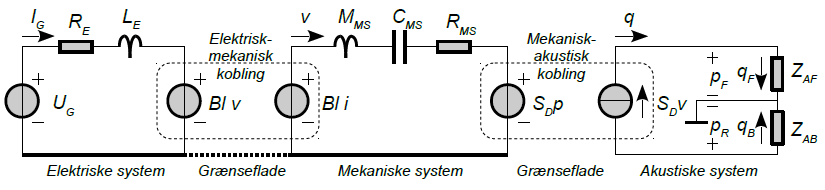
\includegraphics[width=\linewidth]{graphics/30.png}
	\caption{Model af elektro-dynamiske højttaler. \href{http://www.torean.dk/artikel/Elektroakustik.pdf}{(Elektroakustik, TAS)}}
	\label{fig:30}
\end{figure}

\subsection{Snittegning}
\begin{itemize}
	\item Membranen kan kun bevæge sig i akseretningen (lodret). \item For en bashøjttaler kan	bagsidens lydtryk passere gennem huller i rammen og undertiden gennem et hul i magnetens	centerdel.
	\item For en diskanthøjttaler er bagsiden  spærret inde i et lukket rum.
\end{itemize}

\begin{figure} [H]
	\centering
	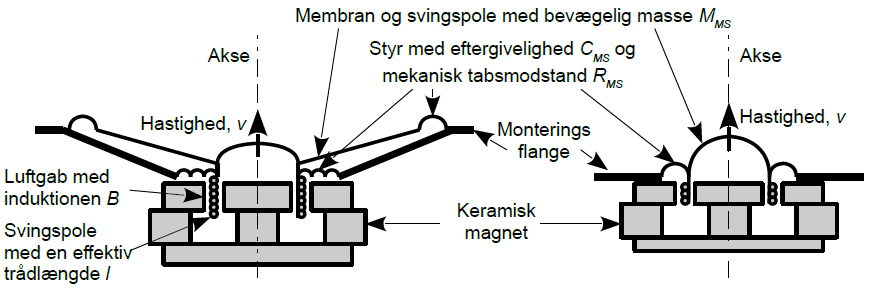
\includegraphics[width=\linewidth]{graphics/22.png}
	\caption{Snit igennem bashøjttaler (venstre) og diskant (højre).\\ \href{http://www.torean.dk/artikel/Elektroakustik.pdf}{(Elektroakustik, TAS)}}
	\label{fig:22}
\end{figure}

\begin{itemize}
	\item Bas
	\begin{itemize}
		\item Model gyldig til cirka \SI{500}{\hertz}
		\item Radius $a = \SI{100}{\milli\meter}$
	\end{itemize}
	\item Diskant
	\begin{itemize}
		\item Model gyldig til cirka \SI{2}{\kilo\hertz}
		\item Radius $a = \SI{12}{\milli\meter}$
	\end{itemize}
\end{itemize}

\subsection{Elektriske system}
\begin{itemize}
	\item Nær kobling mellem systemerne.
	\item Den elektriske impedans afspejler forholdene i det mekaniske- og akustiske system.
	\item Gør det er muligt at måle alle vigtige parametre for alle tre systemer alene fra den elektriske side.
\end{itemize}

\begin{figure} [H]
	\centering
	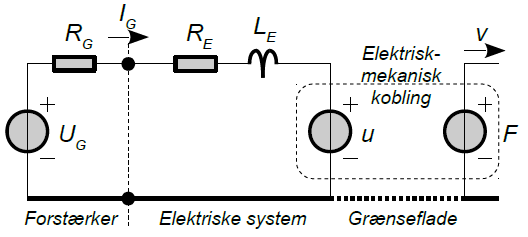
\includegraphics[width=0.8\linewidth]{graphics/23.png}
	\caption{Højttalerens elektriske system. \href{http://www.torean.dk/artikel/Elektroakustik.pdf}{(Elektroakustik, TAS)}}
	\label{fig:23}
\end{figure}
\begin{itemize}
	\item Højttalerens elektriske system består af følgende:
	\begin{itemize}
		\item Effektforstærkeren.
		\begin{itemize}
			\item Repræsenteret ved en spændingskilde $U_G$.
		\end{itemize}
		\item Modstanden $R_E$ fra svingspolens tråd.
		\item Selvinduktionen $L_E$ fra spolens	bevikling.
	\end{itemize} 
	\item Reaktionen fra det mekaniske system beskrives ved:
	\begin{itemize}
		\item Spændingskilden $Blv$ for Faradays induktionslov som følge af den hastighed $v$ svingspolen bevæger sig med.
	\end{itemize}
	\item Højttalerens "\textit{motor}" beskrives ved:	
	\begin{itemize}
		\item Kraftfaktoren $Bl$ hvor $B$ er magnetfeltets induktion og $l$ den effektive længde af tråd der befinder sig i magnetfeltet.
		\item Svingspolens selvinduktion er betydende over frekvensen $f_1$.
	\end{itemize}
\end{itemize}
    
\subsubsection{Typiske værdier}
\begin{itemize}
	\item $U_{G \,RMS}$ = \SI{2.83}{\volt} for \SI{1}{\watt} i nominelt \SI{8}{\ohm} svarer til $U_{G\, PEAK}$ = \SI{4}{\volt}.
	\item $R_E$ = DC modstand af ledningen (\si{\ohm}) typisk \SI{6.4}{\ohm} for \SI{8}{ohm} højtaler.
	\item $L_E$ = Selvinduktion af spolen (\si{\henry}) typisk \SI{1}{\milli\henry} for bas.
	\item $Bl$ = højttalerens kraftfaktor (\si{\tesla\meter}) typisk \SI{10}{\tesla\meter} (\SI{10}{\newton\per\ampere}).
\end{itemize}

\subsection{Mekaniske system}
\begin{itemize}
	\item Den elektrisk-mekanisk grænseflade beskrives ved højttalerens kraftfaktor $Bl$.
\end{itemize}

\begin{figure} [H]
	\centering
	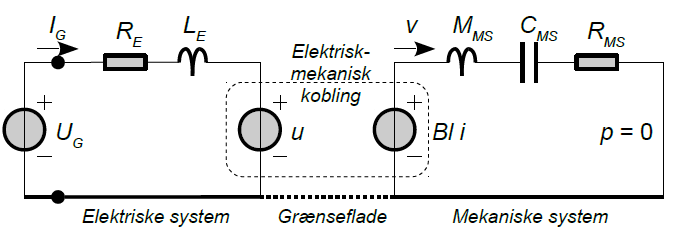
\includegraphics[width=0.95\linewidth]{graphics/24.png}
	\caption{Højttalerens elektro-mekaniske model. \href{http://www.torean.dk/artikel/Elektroakustik.pdf}{(Elektroakustik, TAS)}}
	\label{fig:24}
\end{figure}
\begin{itemize}
	\item Kraften på svingspolen er givet ved højttalerens kraftfaktor og strømmens styrke $F = Bl\, i$.
	\begin{itemize}
		\item Vil accelerere massen af svingspole og membran $M_{MS}$ efter Newtons anden lov. 
	\end{itemize} 	
	\item Styrene fungerer som en fjeder når svingspole og	membran bevæges.
	\begin{itemize}
		\item Trækker svingspole og membran tilbage igen i takt med at
		afstanden øges fra ligevægt.
	\end{itemize} 
	\item Intern friktion i styrene gør at der tabes energi og modelleres ved
	en mekanisk modstand $R_{MS}$. 
	\item Andre tabsmekanismer (dæmpningsmaterialet i kabinettet og den afgivne lydeffekt) kan inkluderes ved at justere på $R_{MS}$.
\end{itemize}

\begin{figure} [H]
	\centering
	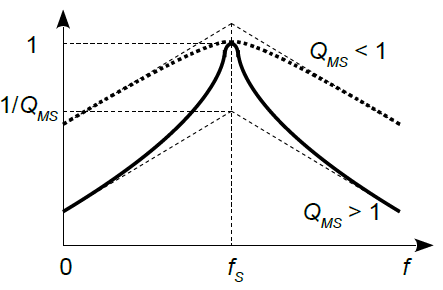
\includegraphics[width=0.5\linewidth]{graphics/26.png}
	\caption{Resonansfrekvensen vil dø ud. \href{http://www.torean.dk/artikel/Elektroakustik.pdf}{(Elektroakustik, TAS)}}
	\label{fig:26}
\end{figure}
\begin{itemize}
	\item Det mekaniske system vil svinge frivilligt hvis det sættes i gang.
	\item Hastigheden er proportional med frekvensen under den mekaniske resonans og den	aftager med frekvensen over resonansen.
	\item $Q_{MS}= \dfrac{1}{R_{MS}}\sqrt{\dfrac{M_{MS}}{C_{MS}}}$
\end{itemize}

\subsubsection{Typiske værdier}
\begin{itemize}
	\item $M_{MS}$ = Masse af bevægeligt system (\si{\kilogram}) typisk \SI{5}{\gram} ... \SI{20}{\gram}.
	\item $R_{MS}$ = Friktionstab (\si{\newton\second\per\meter}) typisk \SI{1}{\newton\second\per\meter}.
	\item $C_{MS}$ = Eftergivelighed af membranstyr (\si{\meter\per\newton}) typisk \SI{1}{\milli\meter\per\newton}.
	\item $f_S$ = Resonansfrekvens (\si{\hertz}) typisk \SI{35}{\hertz}.
	\item $Q_{MS}$ = Godhed af resonans typisk $0.35$.
\end{itemize}

\subsection{Akustiske system}
\begin{itemize}
	\item Den mekanisk-akustiske grænseflade udgøres af membranens areal $S_D$.
\end{itemize}

\begin{figure} [H]
	\centering
	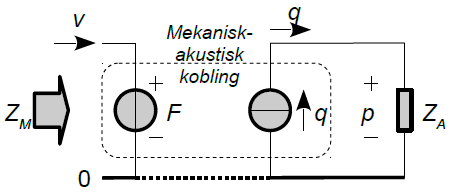
\includegraphics[width=0.65\linewidth]{graphics/25.png}
	\caption{Højttalerens makaniske-akustiske model \href{http://www.torean.dk/artikel/Elektroakustik.pdf}{(Elektroakustik, TAS)}}
	\label{fig:25}
\end{figure}


\subsubsection{Typiske værdier}
\begin{itemize}
	\item $S_D = \pi a^2$ = stemplets areal (\si{\square\meter})
	\item $q = S_Dv$ = volumehastighed (\si{\cubic\meter\per\second})
	\item $Z_A = \dfrac{p}{q}$ = strålingsimpedansen $\left(\dfrac{\si{\newton\meter^{-2}}}{\si{\cubic\meter\second^{-1}}}\right)$
\end{itemize}

\subsection{Thiele-Small parametre}
\begin{itemize}
	\item Højttalerens parametre beskrives i dens datablad som dens Thiele-Small parametre.
	\item Den elektro-mekaniske model kan benyttes til at bestemme værdien af højttalerens parametre.
\end{itemize}
\begin{figure} [H]
	\centering
	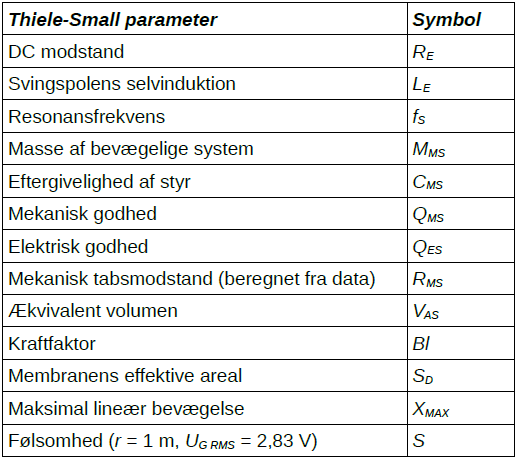
\includegraphics[width=0.85\linewidth]{graphics/27.png}
	\caption{Højttalerens mekaniske-akustiske model \href{http://www.torean.dk/artikel/Elektroakustik.pdf}{(Elektroakustik, TAS)}}
	\label{fig:27}
\end{figure}

\subsection{Elektrisk og mekanisk impedans}
\begin{itemize}
	\item De seriekoblede impedanser fra det mekaniske system optræder nu som parallelkoblede reciprokke	impedanser i serie med svingspolens DC modstand og selvinduktion. 
	\item Impedansen vil have DC modstanden $R_E$ som mindste værdi. 
	\item Der vil være en top på $R_E + R_{ES}$ ved den frekvens $f_S$ hvor
	massen og eftergiveligheden går i resonans.
	\item Impedansen stiger for frekvenser over $f_1$ på grund af svingspolens selvinduktion. 
	\item Resonansfrekvens $f_S = \dfrac{1}{2\pi\sqrt{M_{MS}C_{MS}}}$
	\item Elektrisk impedans $Z_E = \dfrac{u}{i} = \dfrac{(Bl)^2}{Z_M}$
	\item Mekanisk impedans $Z_M = \dfrac{F}{v}= S_D^2Z_A$
	\item $F= S_D p$
\end{itemize}

\begin{figure} [H]
	\centering
	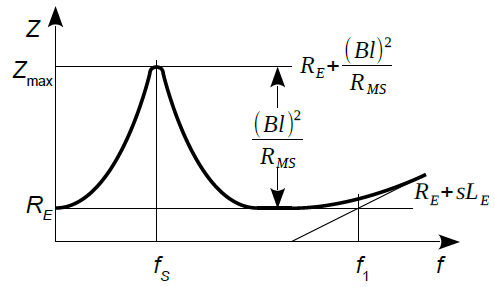
\includegraphics[width=0.7\linewidth]{graphics/28.png}
	\caption{Elektrisk og mekanisk impedans kurve \href{http://www.torean.dk/artikel/Elektroakustik.pdf}{(Elektroakustik, TAS)}}
	\label{fig:28}
\end{figure}

\subsection{Mekanisk og akustisk impedans}
\begin{itemize}
	\item Den akustisk impedans $Z_A$ er givet ved	forholdet mellem lydtryk og volumehastighed.
	\item Volumehastigheden $q$ der er hastigheden af det volumen af
	luft som membranen flytter.
	\item Lydtrykket $p$ der er den kraft luften påvirker membranen med som
	følge af bevægelsen.
	\item Strålingsimpedans $Z_A = \dfrac{p}{q} = \dfrac{Z_M}{S_D^2}$ 
	\item $q = S_D v$
\end{itemize}

\newpage\subsection{Lydtryk}
\begin{itemize}
	\item Højttalerens måleblad benytter et halvt rum.
	\item Højttaleren placeres med målemikrofonen i en afstand på \SI{1}{\meter} fra højttalerens akse.
	\item Effektforstærkeren indstilles til amplituden \SI{4}{\volt} for en effekt på \SI{1}{\watt} ved \SI{8}{\ohm}.
	\item Lydtrykket $p2\pi$ i afstanden $r$.
	\item $|p2\pi|=\dfrac{\rho S_D Bl}{2\pi r M_{MS}R_E}$ 
	\item $L = 20\log_{10}\left(\dfrac{p2\pi_{rms}}{p_{ref}}\right)$
\end{itemize}

\begin{figure} [H]
	\centering
	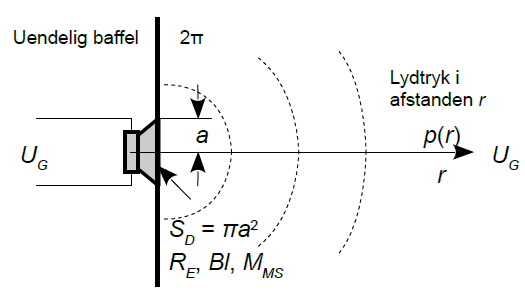
\includegraphics[width=0.7\linewidth]{graphics/29.png}
	\caption{Højttaleren beskrives ved placering i en uendeligt baffel ($2\pi$). \href{http://www.torean.dk/artikel/Elektroakustik.pdf}{(Elektroakustik, TAS)}}
	\label{fig:29}
\end{figure}

\subsubsection{Typiske værdier}
\begin{itemize}
	\item $p$ = amplituden af trykvariationen (\si{\pascal}) typisk \SI{1}{\pascal}.
	\item $r$ = afstanden til mikrofonen (\si{\meter}) typisk \SI{1}{\meter}.
\end{itemize}
\subsection{Øvelser}
\subsubsection{Øvelse 7.1}
Studer modellen med filnavnet: \mintinline{cpp}{PC Loudspeaker.xmcd}. Hvad betyder det at ændre styrets eftergivelighed ($C_{MS}$), det bevægelige systems masse ($M_{MS}$) og den elektriske dæmpning til det dobbelte af den nominelle værdi af $C_{MS}$, $M_{MS}$ og $R_E$. Fx én efter én? 
\newpage \noindent Det vi sigter efter er påvirkningen af resonansfrekvensen, dæmpningsfaktoren $Q$ (godheden) og lydtrykket i det frekvensuafhængige område.

\begin{figure} [H]
	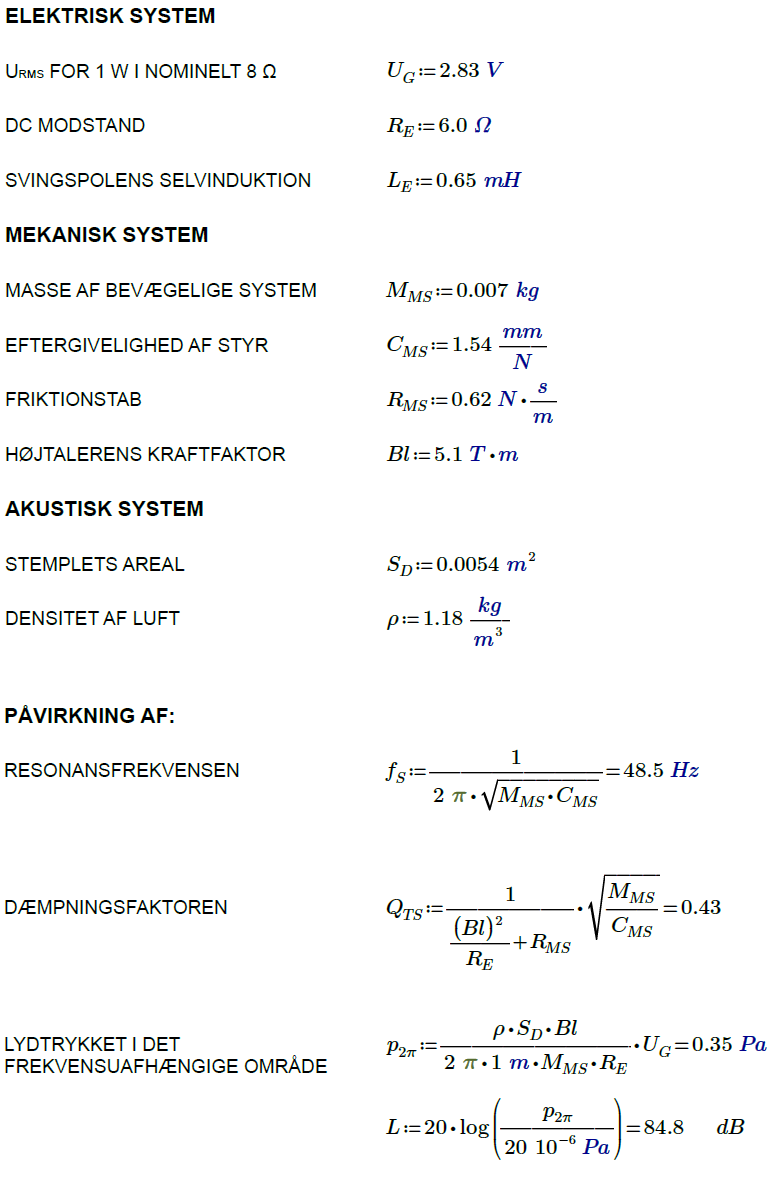
\includegraphics[width=\linewidth]{graphics/31.png}
\end{figure}

\begin{itemize}
	\item Fordobling af den nominelle værdi af 
	\begin{itemize}
		\item $C_{MS}$
		\begin{itemize}
			\item Resonansfrekvensen $f_S$ falder til $\approx\SI{34}{\hertz}$
			\item Dæmpningfaktoren $Q$ ændres til $\approx 0.3$
		\end{itemize}
		\item $M_{MS}$
		\begin{itemize}
			\item Resonansfrekvensen $f_S$ falder til $\approx\SI{34}{\hertz}$
			\item Dæmpningfaktoren $Q$ ændres til $\approx 0.6$
			\item Lydtrykket $L$ falder til $\approx \SI{78}{\deci\bel}$
			\item Der skal mere energi til at systemet svinger
		\end{itemize} 
		\item $R_E$
		\begin{itemize}
			\item Resonansfrekvensen $f_S$ ændres ikke
			\item Dæmpningfaktoren $Q$ ændres til $\approx 0.8$
			\item Lydtrykket $L$ falder til $\approx \SI{79}{\deci\bel}$
			\item Der skal mere spænding til at levere samme strøm
		\end{itemize}
	\end{itemize}
\end{itemize}



\chapter{Højttalerdesign}
\section{Lektion 05-04-2018}

\begin{enumerate}
	\item Højttaler i kabinet
	\item Åben baffel
	\item Lukket kabinet
	\item Basreflex
	\item Slavebas
\end{enumerate}

\begin{mdframed}[style=exampledefault]
	\begin{itemize}
		\item \textbf{Pensum:} 
		\begin{enumerate}
			\item Elektroakustik, TAS,  p. 42-65
		\end{enumerate}
		\item \textbf{Opgaver:} 
		\begin{enumerate}
			\item Lyd og Akustik - Lektion 8 - opgaver og øvelser
		\end{enumerate}
	\end{itemize}
\end{mdframed}

\subsection{Åben baffel}

\subsubsection{Akustisk kortslutning}
\begin{itemize}
	\item Et overtryk på den ene side af membranen vil udligne det tilsvarende undertryk på den anden side.
	\item Ved gengivelse af dybe toner skal lydtrykket fra de to sider af membranen derfor holdes adskilt.
	\item Med et hul i en plade (en baffel) forsinkes og
	dæmpes trykbølgen fra bagsiden.
	\item Herved opstår kun en delvis udslukning af lyden.
\end{itemize}

\begin{figure} [H]
	\centering
	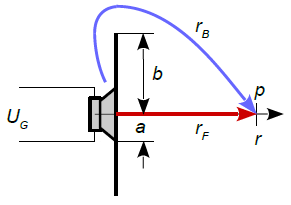
\includegraphics[width=0.5\linewidth]{graphics/53.png}
	\caption{Akustisk kortslutning. \href{http://www.torean.dk/artikel/Elektroakustik.pdf}{(Elektroakustik, TAS)}}
	\label{fig:53}
\end{figure}

\begin{itemize}
	\item Det resulterende lydtryk i afstanden rF beregnes som differensen mellem de to lydtryk.
\end{itemize}

\begin{equation}
p = \dfrac{\rho}{r_F}\dfrac{Bl S_D}{2\pi M_{MS}}\dfrac{U_G}{R_E}\left[1-\dfrac{r_F}{r_B}D(ka)\exp(-jk(r_B-r_F))\right]
\end{equation}


\begin{itemize}
	\item Under	grænsefrekvensen $f_B$ aftager lydtrykket med 6 dB/oktav.
	\item Under højttalerens resonans $f_S$ øges hældningen til 18 dB/oktav. \item Ved høje frekvenser opstår interferens på grund af den skiftende
	fase for bagsidens signal.
	\item Grænsefrekvens $(\lambda/4)$ ved meget stor afstand til mikrofonen.
	\begin{itemize}
		\item Cirkulær baffel med radius $b$.
	\end{itemize}
\end{itemize}

\begin{equation}
f_B=\dfrac{c}{4b}
\end{equation}

\subsubsection{Diffraktion}
\begin{itemize}
	\item Lyden kan ikke uden videre bøjes omkring et skarpt hjørne. 
	\item En kantrefleksion vil	skabe interferens på samme måde som trykbølgen fra bagsiden af højttaleren.
	\item Efter den direkte lyds impuls kommer et svagere og inverteret ekko med en tidsforskel givet ved afstanden fra højttaleren til kanten.
	\item Refleksionskoefficient $R$.
	\begin{itemize}
		\item $R_{Kasse} =−0.33$
		\item $R_{Plade} =−0.50$
	\end{itemize}
\end{itemize}

\begin{figure} [H]
	\centering
	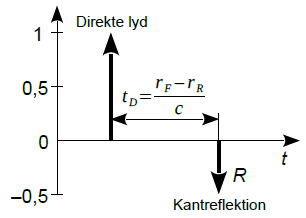
\includegraphics[width=0.5\linewidth]{graphics/54.png}
	\caption{Impulsresponsen for en cirkulær baffel med en punktlydkilde i centrum. \href{http://www.torean.dk/artikel/Elektroakustik.pdf}{(Elektroakustik, TAS)}}
	\label{fig:54}
\end{figure}

\begin{itemize}
	\item Diffraktionen kan beregnes på samme måde som for den akustiske kortslutning ved at addere det direkte bidrag med kantreflektionen.
	\item Det negative fortegn svarer til en subtraktion af det dæmpede og forsinkede ekko fra det direkte signal fra fronten.
\end{itemize}

\begin{equation}
p = \dfrac{\rho}{r_F}\dfrac{Bl S_D}{2\pi M_{MS}}\dfrac{U_G}{R_E}\left[1-\dfrac{r_F}{2r_R}D(ka)\exp(-jk(r_R-r_F))\right]
\end{equation}

\begin{figure} [H]
	\centering
	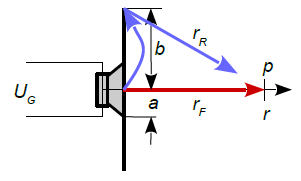
\includegraphics[width=0.5\linewidth]{graphics/55.png}
	\caption{Diffraktion for en cirkulær baffel med radius $b$ og en punktformet lydkilde i centrum. \href{http://www.torean.dk/artikel/Elektroakustik.pdf}{(Elektroakustik, TAS)}}
	\label{fig:55}
\end{figure}

\subsection{Lukket kabinet}
\begin{itemize}
	\item Eliminere udstrålingen fra bagsiden ved at montere højttaleren i et lukket kabinet for effektivt at holde de to sider adskilt.
	\item Den indespærrede luftvolumen $V_B$ udgør en eftergivelighed $C_{AB}$ som	belaster membranens bagside.
	\item En vigtig specifikation for en højttaler er dens ækvivalente volumen $V_{AS}$.
	\item En højttaler med resonansen \SI{50}{\hertz} monteres i et kabinet med samme volumen som $V_{AS}$ specifikationen vil resonansen hæves 1.4
	gange til \SI{70}{\hertz}.
\end{itemize}

\begin{figure} [H]
	\centering
	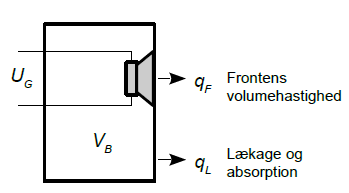
\includegraphics[width=0.5\linewidth]{graphics/59.png}
	\caption{Lukket kabinet. \href{http://www.torean.dk/artikel/Elektroakustik.pdf}{(Elektroakustik, TAS)}}
	\label{fig:59}
\end{figure}
\begin{itemize}
	\item Det resulterende lydtryk for et lukket kabinet.
\end{itemize}
\begin{figure} [H]
	\centering
	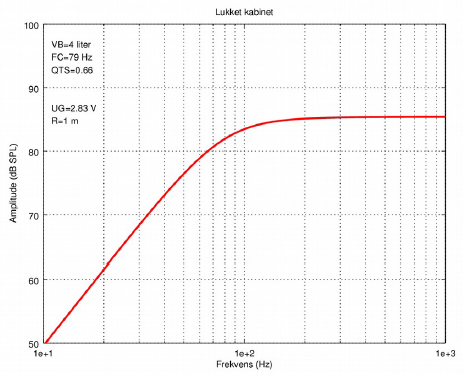
\includegraphics[width=0.75\linewidth]{graphics/58.png}
	\caption{Lukket kabinet. \href{http://www.torean.dk/artikel/Elektroakustik.pdf}{(Elektroakustik, TAS)}}
	\label{fig:58}
\end{figure}


\subsection{Basreflex}
\begin{itemize}
	\item Udnyttelse af effekten fra højttalerens bagside til at støtte basgengivelsen i et mindre frekvensområde ved et såkaldt ventileret kabinet.
	\item Massen af luften i porten danner en resonans	med det indespærrede luftvolumen.
	\item Massen af luftproppen i porten beregnes som massefylden af luft $\rho_0$ gange med luftvoluminet der er arealet af porten $S_P$ ganget med længden af porten $L_P$.
	\item Den omregnes til akustisk masse $M_{AP}$ ved division med $S_P$ kvadreret
\end{itemize}

\begin{equation}
M_{AP}=\dfrac{\rho_0}{S_P}(L_p+1.5\sqrt{\frac{S_P}{\pi}})
\end{equation}

\begin{itemize}
	\item $\rho_0 = \SI{1.18}{\kilogram/\meter\cubic}$
\end{itemize}

\begin{figure} [H]
	\centering
	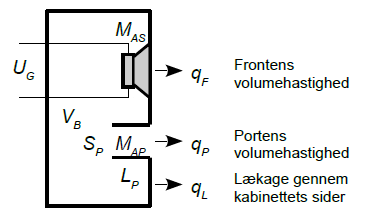
\includegraphics[width=0.5\linewidth]{graphics/56.png}
	\caption{Et basreflex kabinet inkluderer en port. \href{http://www.torean.dk/artikel/Elektroakustik.pdf}{(Elektroakustik, TAS)}}
	\label{fig:56}
\end{figure}
\begin{itemize}
	\item Rød kurve er det resulterende lydtryk.
	\item Grøn kurve er	lydtrykket fra højttalerenheden.
	\item Blå kurve viser hvor meget port står for.
\end{itemize}

\begin{figure} [H]
	\centering
	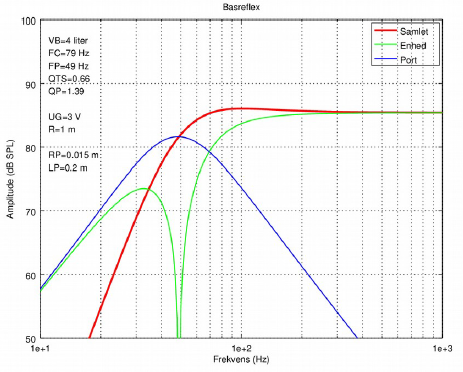
\includegraphics[width=0.75\linewidth]{graphics/60.png}
	\caption{basreflex kabinet. \href{http://www.torean.dk/artikel/Elektroakustik.pdf}{(Elektroakustik, TAS)}}
	\label{fig:60}
\end{figure}

\subsection{Passiv slave}
\begin{itemize}
	\item Erstatter porten med en passiv højttaler, kaldet en slavebas.
	\item En højttaler med membran og styr, men uden magnet og svingspole.
	\item Portens masse $M_{AP}$ erstattet af højttalerens $M_{AS}$, $C_{AS}$ og $R_{AS}$.
\end{itemize}

\begin{figure} [H]
	\centering
	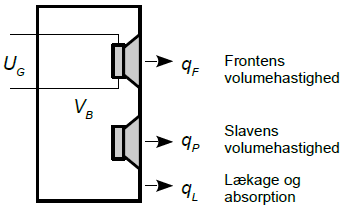
\includegraphics[width=0.5\linewidth]{graphics/57.png}
	\caption{Et kabinet med en passiv slave. \href{http://www.torean.dk/artikel/Elektroakustik.pdf}{(Elektroakustik, TAS)}}
	\label{fig:57}
\end{figure}

\begin{itemize}
	\item $M_{AS}=\dfrac{M_{MS}}{S_D^2}$
	\item $R_{AS}=\dfrac{R_{MS}}{S_D^2}$
	\item $C_{AS}=C_{MS}S_D^2$
\end{itemize}

\begin{itemize}
	\item Rød kurve er det resulterende lydtryk.
	\item Grøn kurve er	lydtrykket fra højttalerenheden.
	\item Blå kurve viser hvor meget slave står for.
\end{itemize}

\begin{figure} [H]
	\centering
	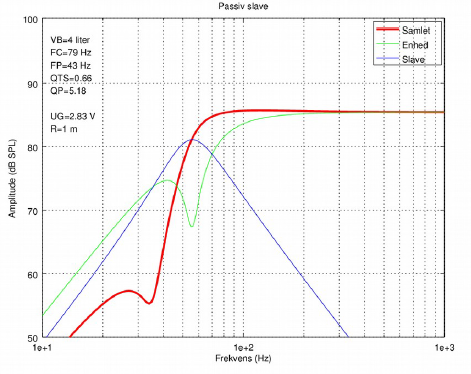
\includegraphics[width=0.75\linewidth]{graphics/61.png}
	\caption{basreflex kabinet. \href{http://www.torean.dk/artikel/Elektroakustik.pdf}{(Elektroakustik, TAS)}}
	\label{fig:61}
\end{figure}

\subsection{Øvelser}
\subsubsection{Øvelse 8.1}
Design et anden ordens delefilter for et tovejs system med en bas og diskanthøjttaler med udgangspunkt i formlerne fra noten \href{http://www.torean.dk/artikel/Elektroakustik.pdf}{Elektroakustik, s. 82}. Find et par højttalere på nettet og benyt de rapporterede frekvenskarakteristikker og øvrige data for de valgte enheder til at finde en egnet delefrekvens. \\

\noindent Beslut om diskanthøjttaleren skal ompoles (inverteres) eller forskydes mekanisk på fronten for at få en korrekt faserelation mellem enhederne. \\

\noindent Vælg godheden Q for hver gren af delefiltret. Beslut om der skal korrigeres for bashøjttalerens stigende impedans (s. 37) og for diskanthøjttalerens resonans, og beslut om diskanten skal dæmpes for at passe til bashøjttaleren (s. 85). Begrund de trufne valg!



\chapter{Lyddæmpning og lyddiffusion}




\end{document}